\par
\par
\par
Answer: 2, 12, 48\\
\textbf{Proof.} First we give each vertex of graphs an ID for convenience.
\begin{figure}[hpbt]
\begin{center}
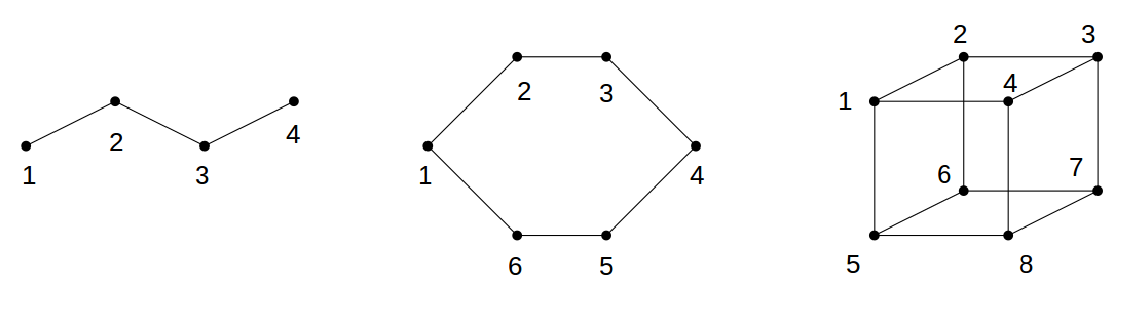
\includegraphics[width=0.8 \textwidth]{ex6-1_img.png}
\end{center}
\end{figure}

In the first graph, there are two vertex $1,4$ with only one degree, which means their corresponding vertices in automorphism have only one degree. Therefore we have 
$$f(1)=1, f(4)=4$$ 
or 
$$f(1)=4, f(4)=1$$
Either case the automorphism can be determined. There are $2$ automorphic graphs. The functions are
$$f_1=\{\{1,1\}, \{2,2\}, \{3,3\}, \{4,4\}\}$$ 
$$f_2=\{\{1,4\}, \{2,3\}, \{3,2\}, \{4,1\}\}$$
\par In the second graph, we take vertex $1$ and $2$ and the edge between them $e_{12}$. The corresponding edge in the automorphism can be $e_{12},e_{21}, e_{23}, e_{32},..., e_{61},e_{16}$. Once the corresponding edge of $e_{12}$ is determined, the automorphism is determined. So there are  $12$ automorphisms.

\par In the third graph, we will illustrate our methods by an example first. If we take $e_{12}$ and choose $e_{43}$ as its mapping in automorphism, there are $4$ choices left for $e_{14}$, as $e_{14}$ can be $e_{14}, e_{23}, e_{48}, e_{37}$. Once the mappings of $e_{12}$ and $e_{14}$ are determined, the automorphism is determined. We have $12$ choices for $e_{12}$ and $4$ choices for $e_{14}$, so there are $48$ automorphisms.